\section{Этап Post-process} \label{ch3:post_process}
	\begin{figure}[ht!] 
		\center
		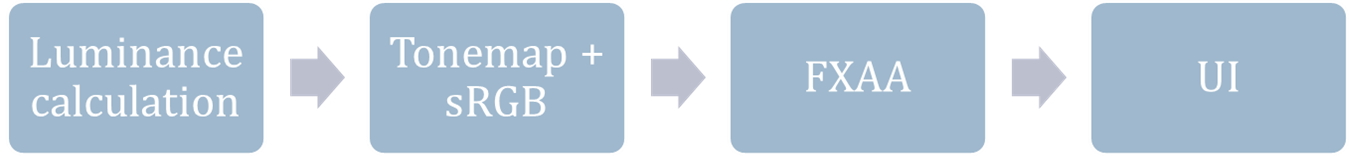
\includegraphics [scale=0.4] {my_folder/images//postprocess_schema}	
		\caption{Схема этапа Post process предлагаемого конвеера.} 
		\label{fig:renderpass_schema}
	\end{figure}
	
	На данном этапе, происходит пост-обработка кадра, получившегося на предыдущем этапе. В качестве пост-обработки предлагаются:
	\begin{enumerate}[1.]
		\item Алгоритм Filmic Tonemapping\cite{hable2010uncharted}
		\item Алгоритм Fast Approximate Anti-Aliasing\cite{lottes2009fast}
	\end{enumerate}

	Данный этап не притерпевает каких-либо изменений, при использовании предлагаемого алгоритма непрямой отрисовки, потому что на данном этапе не используются объекты сцены.